\chapter{回到康熙早年}
% 原书第149页

关于索额图获罪，并不是没有留下其他的说法，只是这个说法与传统熟知的记录差别很大，没有受到过重视。在清史学者们熟知的《读书堂西征随笔》（后文简称《西征随笔》）中就有记录：


% 原书第149页

\begin{bookquote}索额图死于宗人府，籍没赀财，全家受祸，皆高为之。\end{bookquote}

% 原书第149–150页

这里提到的“高”是指康熙身边的南书房近侍高士奇。高士奇以书画闻名后世，在现今各种拍卖会中经常能看到他的作品。高士奇借宫廷任职之便，以及在书画圈子中的各种关系，见到了历史上很多书画真品，写下了《江村销夏录》这部评点古代重要书画的专著。他的评点和提供的信息在书画史以及现今书画鉴定中都有重要地位。\NoteRef{05}{1}


% 原书第150页

高士奇在他的时代真正被举国上下称奇的是，他只考过了秀才，却被特别提拔入南书房，供奉内廷，授职翰林院，与一帮当时通过科举入朝、最不可一世的士子平起平坐。而且高士奇还一直特别受到康熙的垂青。他死后，康熙赐给他了“文恪”的谥号。康熙在赐给高士奇谥号前，还向群臣坦言，自己知道按规矩高士奇不应该有谥号，赐谥是破例。\NoteRef{05}{2}当时士子对高士奇的心态，是羡慕和嫉妒并存，这在许多文人文集中提到他时都能感觉到。


% 原书第150页

有了这个背景，才好理解为什么比高士奇（1645—1703）小二十七岁的汪景祺（1672—1726）会在《西征随笔》中专门写到他。汪景祺是年羹尧的幕僚，书名中所谓的“西征”就是雍正初年年羹尧的西征。从学历上看，汪景祺是举人，比高士奇的秀才要高一个档次，但他两人又都没能考得进士出身。汪景祺是个不安于现状，想在政治圈掀起风浪的人。他通过私人关系，专门去往西北，拜在当时正如日中天的年羹尧门下，希望从做幕僚开启仕途。


% 原书第150–151页

与索额图有关的内容，在《西征随笔》一书“张汧、祖泽深之狱”及“高文恪遗事”相邻的两章内。根据汪景祺的记录，高士奇最早到北京时，是在报国寺的廊下卖字糊口，“秃笔破砚”，很是可怜。有一天，来报国寺的吏部主事（六品）祖泽深遇到了高士奇，成了他的贵人。在汪景祺笔下，祖泽深是个贪官，但是他会相面，看出了高士奇大贵，有宰相之相，因此把高士奇收为弟子。在他的引荐下，高士奇凭借一笔好字，以及善于察言观色的本事，进入索额图家做幕僚。再后来，索额图把他推荐给了康熙。


% 原书第151页

在正史中，高士奇确实是康熙信任的人。尽管高士奇官位不高，但是他时刻都在皇帝的身边，是天下官员争相攀附的对象。这一点是历史中已知的部分。而《西征随笔》提供的不为人知的部分则是索额图对高士奇始终“以奴视之”，而且每次高士奇见到索额图都需要“长跪启事”。汪景祺还写下了一个生动的例子来反映二者之间的主奴关系。1703年，也就是索额图被康熙治罪的那一年，有一天，索额图没穿衣服坐在椅子上，对着跪在地上，而且额头已叩在地面的高士奇破口大骂，骂的内容还“辱及父母妻子”。当时的高士奇已经是名满天下之人。对于这样的场景，汪景祺说连在索额图家的门客看到后都赶紧回避，怕高士奇知道自己看到了，以后寻机报复。同时，汪景祺还提到让高士奇忍无可忍的，是索额图门下一位叫江黄的人。这位江黄是绍兴人，颇受索额图重视，和他的主子一样，也蔑视高士奇。在汪景祺的故事逻辑中，来自索额图家的蔑视是高士奇决定要报复举荐过他、对他有恩的索额图的原因。故事的结尾是高士奇通过投靠索额图的朝堂宿敌明珠，把索额图扳倒了。


% 原书第152页

\begin{figure}[htbp]\centering
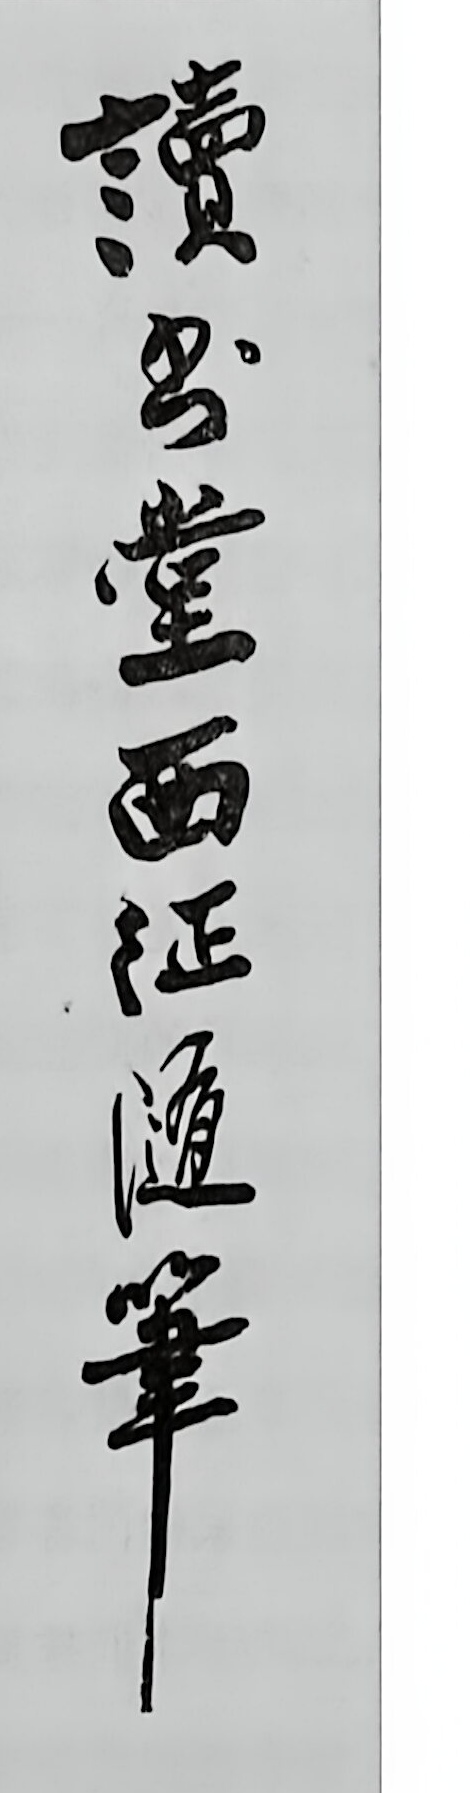
\includegraphics[width=.9\linewidth,height=.68\textheight,keepaspectratio]{assets/fig-172a.jpg}
\caption{疑为汪景祺自题书名}\label{fig:172a}\end{figure}
\begin{figure}[htbp]\centering
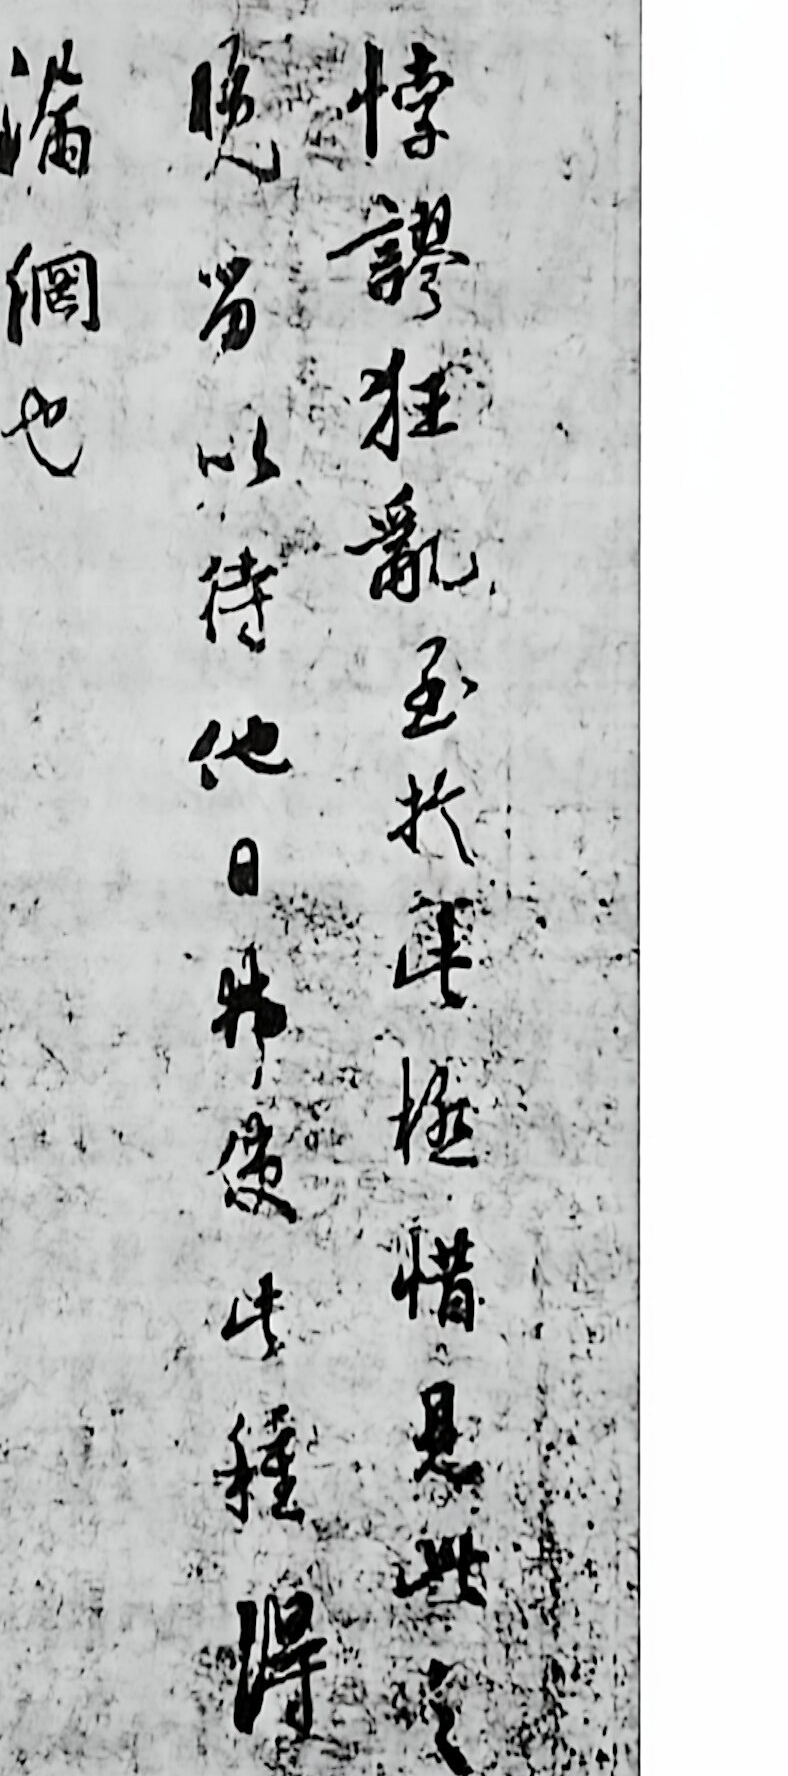
\includegraphics[width=.9\linewidth,height=.68\textheight,keepaspectratio]{assets/fig-172b.jpg}
\caption{雍正在《西征随笔》卷首所作御批}\label{fig:172b}\end{figure}


% 原书第153页

汪景祺所写的内容与我们现下流行的对索额图案的解释完全不同。在汪的版本中，索额图的倒台跟谋反、储位这些没有关系，而是栽在了历史上最常见的人事争斗中。对于后来读史的人来说，大概第一个问题就是汪景祺写的东西可信吗？也就是说，《西征随笔》是一本可以用来了解朝堂历史的书吗？


\begin{sectionnotes}

% 原书注释：原书第405页
\BookNote{05}{1}{高士奇书画方面历史参看励俊，《追寻江村秘藏：高士奇书画鉴藏与流散研究》；钟国豪，《清初文臣高士奇（1645—1703）绘画鉴藏品味研究》。}

% 原书注释：原书第406页
\BookNote{05}{2}{《圣祖仁皇帝实录》，卷219。}

\end{sectionnotes}
\section{《西征随笔》的由来}

% 原书第153页

《西征随笔》在后世出名并不是因为其讲述的朝野掌故，而是作为年羹尧案的一部分，同时其作者汪景祺也因书致祸。在有些研究中，这本书是清初文字狱的一个案例。雍正因为这本书，对汪景祺的处罚很严酷：将其枭首示众；妻和子都被流放到黑龙江，给当地贫穷兵丁做奴隶；兄弟亲侄被革职，发往宁古塔；五服以内的族人在职以及在候补职位的俱行革职，送回原籍，由地方官管束。这本书给汪景祺整个家族都带来了灾难。汪景祺的人头从1726年被斩首后就挂在北京菜市口，一挂就是十年，到了1735年，还有官员上书乾隆，称京城是“首善之区”，人头挂在闹市，实在有碍“观瞻”，请求取下掩埋。\NoteRef{05}{3}


% 原书第153–154页

《西征随笔》是汪景祺写给年羹尧的手写书稿，并没有在民间流传过。书稿是在年羹尧被贬到杭州后，查抄其住所时发现的。手写本上交给雍正后，就一直存在宫中。民国时，据发现《西征随笔》的故宫学者许宝蘅记录，最早是在懋勤殿（乾清门附近）一口锁着的箱子中发现了这本书。\NoteRef{05}{4}这本书的卷首还有当年雍正的御批：


% 原书第154页

\begin{bookquote}悖谬狂乱，至于此极。惜见此之晚。留以待他日，弗使此种得漏网也。\NoteRef{05}{5}\end{bookquote}

% 原书第154页

《西征随笔》在民国年间被发现时，原本的上下两卷只存有上卷（约三万四千一百字）和下卷中的一篇，外加一首诗（约一千二百五十字）。留存部分其实看不出来雍正所谓的“悖谬狂乱至于此极”。《西征随笔》从1928年开始陆续连载于《掌故丛编》。同年，又以专书形式影印出版。在推出影印本的时候，许宝蘅已经对该书做过一些考证，提出现存《西征随笔》并不是雍正看到的全本，因为雍正朝《实录》提到过《西征随笔》里的一些内容在现存的手稿中没有。比如雍正在处理后来的查嗣庭案时，提到过《西征随笔》中的一些内容，但这些内容不见于现存部分。另外一个更明显的例子，雍正朝《实录》还全文引用过《西征随笔》记载的“程如丝贪横”案，但这个贪腐案也不见于故宫发现的《西征随笔》手稿。\NoteRef{05}{6}也就是说，现在看到的《西征随笔》下卷的大部分内容已经被销毁了。


% 原书第155页

到底被删除部分中的内容有多“悖谬”，已经不得而知，可以知道的是，刑部等部门商议后，给汪景祺写《西征随笔》的处罚决定是：“照大不敬律，拟斩立决。”给出的理由很简单：“汪景祺作诗讥讪圣祖仁皇帝。”\NoteRef{05}{7}这一条罪名成为了从许宝蘅开始，所有现当代学者阅读《西征随笔》时的主要关注点。纵观全书，汪景祺多次提到过“先帝”，都是很尊敬的口吻；只是在书中“诙谐之语”一章，讲到了一则涉及康熙的故事。有一位叫杜诏的生员，在路旁迎接南巡的康熙并献诗；康熙高兴之余，赐给杜诏一首题写在绫上的《春日偶成》：


% 原书第155页

\begin{bookquote}云淡风轻近午天，傍花随柳过前川。时人不识予心乐，将谓偷闲学少年。\end{bookquote}

% 原书第155页

杜诏得到御赐后，回乡给众人炫耀。其中一人看到这幅题字，也写了一首诗：


% 原书第155页

\begin{bookquote}皇帝挥毫不值钱，献诗杜诏赐绫笺。千家诗句从头写，云淡风轻近午天。\end{bookquote}

% 原书第155–156页

宋代理学家程颢的《春日偶成》是古代儿童诗歌启蒙选编《千家诗》的第一首，所以“皇帝挥毫不值钱”、“千家诗句从头写”有诙谐之处，汪景祺便把其写入了《西征随笔》“诙谐之语”一章。笔记以诙谐为题专列一章，其实是《世说新语》的成法，在传统文人笔记中常见。但也不可否认，这首诗确有对康熙讥讪的意味。不过，当这句诗的“讥讪”成为了后世对这本书的概括，也就等于将其视为一本文人戏谑的笔记，从而忽视了其特有的史料价值。


% 原书第156页

更重要的问题在于，这句诗真是雍正看到《西征随笔》后愤怒的原因吗？这就是雍正所谓的“悖谬狂乱”之极吗？现存《西征随笔》下卷只有一篇文章和一首诗，是不是真正“悖谬狂乱”之言已经被销毁了？


% 原书第156页

除了雍正看到这本书后留下的御批文字以外，故宫档案中还有一份发现《西征随笔》的官员给雍正上的密折。这份密折为后世了解这本书的发现经过提供了丰富的细节。


% 原书第156–157页

杭州的傅敏和鄂弥达在雍正三年十月十七日（1725年11月21日）用汉文密折上报雍正，详细讲述了发现《西征随笔》的经过：九月二十八日下午四五点，雍正派的钦差阿拉锡（满文奏折翻译中又作拉锡）从北京来到杭州，找到时任浙江巡抚的傅敏（满文奏折翻译中又作福敏）和杭州将军的鄂弥达，告知这两位杭州最高级别的文武官员，他是来传旨缉拿年羹尧回京的。当时的年羹尧已是穷途末路，被贬为了杭州城东门守卫。两位地方官不敢怠慢，当晚就与阿拉锡一道找人把在城门值夜的年羹尧召来，由傅敏向年羹尧宣读了谕旨，然后将其锁拿。傅敏是乾隆的老师，是长期在雍正府上的人。从政治派系上来说，他和年羹尧同为雍正藩邸旧人，属于雍正私人圈子里的人。\NoteRef{05}{8}谕旨由他来宣读，年羹尧也无话可说。雍正已提前安排好，这次缉拿回京就是年羹尧的终点。所以在年被锁拿后，接着就是抄家。阿拉锡写了几份满文密折，详细说明了他遇到年羹尧后的所见所闻，以及抄家所获的物件。\NoteRef{05}{9}而由傅敏主笔的汉文密折（鄂弥达主要使用满文上密折），专门提到了《西征随笔》是在阿拉锡离开抄家现场以后，他们在后续详细搜查时发现的。这也解释了为什么单单这件抄来的物品是由他们报告：


% 原书第157页

\begin{bookquote}阿拉锡起身之后，臣等再加细搜粗重家伙，于乱纸中得抄写书二本。书面标题《读书堂西征随笔》，内有自序，系汪景祺姓名。臣等细观其中所言，甚属悖逆，不胜惊骇，随连日密访其人……\end{bookquote}

% 原书第157页

傅敏还在密折中告知雍正，根据年羹尧的家人招供，年在此前已把各类书信都烧掉了。这变相向雍正解释了为什么他们在抄家过程中只发现了《西征随笔》这一本让他“惊骇”的文字材料。他对《西征随笔》还有评论：


% 原书第158页

\begin{bookquote}年羹尧蒙国厚恩，若无悖逆之心，谁敢以此诽谤妖言达于其侧……\end{bookquote}

% 原书第158页

然后，傅敏又写了很长一段话来狠批年羹尧是如何的大逆不道，竟然敢收藏这本书。傅敏在结尾写道：


% 原书第158页

\begin{bookquote}臣等受恩深重，义不与逆贼共戴天日。\NoteRef{05}{10}\end{bookquote}

% 原书第158页

傅敏用了整个密折三分之一的篇幅来批判年羹尧敢于收藏这本书的罪过。传统中杀父之仇才是不共戴天，而年羹尧藏了一本书，傅敏就表示与他不共戴天，可以想见傅敏看到内容后的“惊骇”程度。表面上看，批判年羹尧的文字似乎是傅敏对年羹尧落井下石，是人品问题。但是细思之下，更展现了傅敏对于自己看到了书中内容后所感到的恐惧，以至于需要用这样的批判来与之划清界限。这种恐惧之情在阿拉锡的满文奏报中也有体现。阿拉锡把各种抄家收到的物品一件一件详细描述，各种金银珠宝、西洋物件的尺寸大小都做了详细汇报，唯独对文字材料连看都不敢看：


% 原书第158–159页

\begin{bookquote}其书房房檐下钉有木夹之书。奴才拉锡、鄂弥达、福敏我等三人原欲开阅，后奴才虞其有何关联之处，遂派人问年羹尧，伊告曰“木板所夹者乃谕旨也”等语，故而未看。\NoteRef{05}{11}\end{bookquote}

% 原书第159页

他们奉旨抄家，却连发现的文字材料看都不敢看，可见三人的警觉。在整个收缴《西征随笔》的过程中，傅敏是第一个看到这本书的人。从他看到这本书后给出的评价，以及他表现出的“不胜惊骇”，他看到的内容，应该不是我们现代人所见的“皇帝挥毫不值钱”这样一句戏谑之言。大概率是书里有臣子不可与闻的宫廷秘闻，还很有可能关系到了雍正。


% 原书第159页

雍正看到傅敏的密折和送来的《西征随笔》后所做朱批，也说明了书里有不能流传后世的内容。雍正叮嘱傅敏：


% 原书第159页

\begin{bookquote}此奏甚属可嘉，将此两本内朕不曾令发出。尔等见此书内言辞之人，亦当密之可也。\NoteRef{05}{12}\end{bookquote}

% 原书第159页

他告诉傅敏，两卷本的《西征随笔》他没在朝廷公布，同时也命傅敏等见过这书的人要对内容保密。\NoteRef{05}{13}


% 原书第159–160页

在提到《西征随笔》时，现当代研究有一个根本性的误区，就是将其与年羹尧案相关联，把对它的研究置于年羹尧案中来进行，进而背离了这本书原本具有的价值。一旦了解这书的发现过程，就知道这本书本质上跟年羹尧案没有关系。由于前人对《西征随笔》的解读总是从年羹尧案入手，因此只能看到其中一些对年羹尧的肉麻吹捧。像前面章节中提到的，汪景祺称赞年是“宇宙第一伟人”就出自这本书。这句话大概是《西征随笔》中被引用最多的一句。雍正要处置、缉拿年羹尧早有决定，只是意外发现了《西征随笔》，这本书便成为了年羹尧九十二条罪状之一。但其实有没有这本书，年羹尧案的结局都不会有任何不同。汪景祺和《西征随笔》惹怒雍正的，是里面记录了不应该记录的朝堂之事。


% 原书第160–161页

《西征随笔》是身为幕僚的汪景祺写给幕主年羹尧参用的。他在写这本书的时候，年羹尧正如日中天，因而汪的目的是要展现自己作为幕僚的价值。具体说来，汪要展示的是他对北京官场的熟悉，对个中脉络的掌握。幕僚这一功能在《红楼梦》“葫芦僧乱判葫芦案”一回门子如数家珍般介绍当地官场的描绘中已为人所熟知，在此不再展开。\NoteRef{05}{14}《西征随笔》本质上是汪景祺向年羹尧展示其知晓那些没摆在明面上的朝廷轶事，以及这些事情来龙去脉的一本书。还有一点需要注意，尽管年羹尧以“抚远大将军”的身份平乱西北，名垂后世，但年羹尧本质上是个文臣，是康熙三十九年（1700）的进士。他先是在翰林院里跟文臣们历练多年，后来又被康熙派去四川做巡抚。在做大将军前，年羹尧在中央和地方上都摸爬滚打过，是一个既能治理地方，又能统帅三军的人。像索额图、高士奇这些在《西征随笔》中写到的人物，都是年羹尧早年在翰林院里打过交道，最起码也是有所耳闻的人物。因而当汪景祺给年羹尧讲北京官场旧事的时候，他写出来的东西是需要有可信度的。用今天的话说，他这本书是写给内行看的。书中提到张鹏翮长相娇媚，像戏旦。而张鹏翮是年羹尧的同僚，二人同为进士出身。张长什么模样，年羹尧是知道的。就在《西征随笔》成书前一两年，年羹尧在最后一次面见康熙（1721）后，还向康熙推荐张鹏翮去治理河道。另外，像上面提到书中的程如丝贪污案。程如丝就是四川官员，是年羹尧手下之人。所以，对年羹尧来说，《西征随笔》并不是一本历史书。当然《西征随笔》有吹捧年羹尧的话，这不假；吹捧的话术是政治圈中的常态。现存绝大多数给皇帝的密折里，都包含着各种肉麻的吹捧；但对后来读史的人来说，重要的不是那些吹捧，而是那些谈正事的部分。我们不会因为密折中有吹捧的话术，就低估了这些密折的价值。同样，如果我们只看到《西征随笔》中吹捧年羹尧的话，那就是买椟还珠了。


% 原书第161–162页

尽管汪景祺被雍正杀了，《西征随笔》也被封锁，没有流传，但肯定这本书史料价值的恰恰是雍正自己。大约一年后，查嗣庭案爆发，雍正又提起了汪景祺，还把查、汪二人做对比。海宁查氏是江南望族，明清年间该家族进士辈出，金庸（原名查良镛）成名后还曾回海宁祭祖。查嗣庭是康熙四十五年（1706）的进士，官至礼部侍郎。他的案子很复杂，是在康熙皇八子、皇九子去世大概一两个月后爆发，至今学界对当时的朝廷气氛以及各种关系都不是很清楚。但根据官方记载以及从表面上看，该案是查嗣庭在文字上被抓住了把柄，写了雍正认为不应该写的东西，并被查了出来：


% 原书第162页

\begin{bookquote}狂妄无忌惮之徒，往往腹诽朝政，甚至笔之于书，肆其诬谤。如汪景祺、查嗣庭，岂能逃于天谴乎？\NoteRef{05}{15}\end{bookquote}

% 原书第162页

这是在查嗣庭案期间雍正所作的评价。在雍正的逻辑里，汪景祺和查嗣庭犯的是相同的问题：把“腹诽”，也就是心里的不满，写了出来。在抄查嗣庭家的时候，发现了他写的日记。雍正点评说：


% 原书第162页

\begin{bookquote}其日记所载狂妄悖逆之语，与汪景祺相为表里。而其诽议圣祖仁皇帝用人行政，大逆不道之言，不可胜举。\NoteRef{05}{16}\end{bookquote}

% 原书第162–163页

也就是说，在雍正眼里，查嗣庭和汪景祺他们写下来的东西，核心问题是“诽议”了康熙时期的用人行政，记录了雍正认为他们不应该写下来的事。这个说法其实最能解释傅敏看到《西征随笔》后所谓的“不胜惊骇”。他“惊骇”的是写下来的具体事情，而不大可能是“皇帝挥毫不值钱”这样无关痛痒的文人戏谑。


% 原书第163页

通过上面雍正的评述可以看出，汪景祺所写和查嗣庭所记，在雍正那里属于同一个类型：不该记录之事。但同时需要注意的是，他们并不是编造的。这一点并非后来人的逻辑推理所得，反而是出自雍正自己对《西征随笔》内容的评价。他在后来的朝堂审案中，还提起过《西征随笔》记载之事，并且告诉朝臣这是调查案件的线索。雍正在查办夔州知府程如丝贪污案时，全文引用了《西征随笔》中“程如丝贪横”一节的记载。雍正当时宣谕的对象是“大学士”和“九卿”等，大概他也觉得引用被他杀了的汪景祺的文字作证似乎有点不妥，于是最后借用孔子的话来给自己打圆场：


% 原书第163页

\begin{bookquote}孔子曰：君子不以人废言。汪景祺虽犯重罪，身正典刑，然其言未必字字皆虚。\NoteRef{05}{17}\end{bookquote}

% 原书第163页

雍正在要杀汪景祺时，批《西征随笔》悖逆，但实际上他自己是认真读过这本书的。杀掉汪两年后，他还能记得书里的内容，并切实用来查案。但他引用的程如丝贪横部分，又被他或者后来清宫中的人删除了，并不见于民国发现的《西征随笔》。


% 原书第163–164页

除了汪景祺自己，《西征随笔》的两卷全本只有少数几个人看过。其中可以明确的是：年羹尧、傅敏和雍正三人。无论从文化上说，还是就官场政治的熟悉程度来讲，这三人都是当时最有资格评价这本书的人。他们三人一致对这本书很重视。就算傅敏和雍正用的是批判的语气，也能看出二人认定这本书不能轻忽。


% 原书第164页

汪景祺在书中称呼康熙为先帝，也就是说《西征随笔》是在康熙去世后（1722年12月）到年羹尧倒台前（1725年）这段时间写出来的，或者更准确地说可能是在年羹尧西征结束（1724）后完稿的。其成书时间比我们看到的康熙朝《实录》更早，因而其撰写内容没有受到过雍正朝那些编订康熙朝《实录》的翰林们的影响，是完全独立的创作路径。


% 原书第164–165页

另外，汪景祺也不是一个没有背景的普通举人。他出自官宦世家，是真正身处北京官场的人。汪景祺原名汪日祺，是户部侍郎汪霦次子。而汪霦是康熙十五年（1676）进士，做过翰林院编修。\NoteRef{05}{18}在桐城派大师方苞纪念李光地的文章中，曾经提及康熙说到：“自汪霦死，无能古文者。”在这种情况下，李光地给康熙推荐了方苞。\NoteRef{05}{19}在发现《西征随笔》时，汪景祺的亲哥汪见祺在做礼部主事。而在朱彝尊的诗中，也提到过他曾经与汪霦和汪景祺聚会过。根据故宫发现《西征随笔》的学者考证，朱彝尊的诗在雍正朝之后刊刻的版本中，已经把汪景祺的名字去掉了。也就是说汪景祺案后，他们汪家的很多资料已经不存在了。即便如此，也已经可以看出汪景祺并非寻常举人。


% 原书第165页

汪景祺正因为有这样的背景，才会被年羹尧和雍正重视。准确地说，汪景祺是以自己特有的人脉和经历，在书写一些并不会出现在正史里的内容。当然汪也知道很多东西是不能写出来的，他在序言中也写道：


% 原书第165页

\begin{bookquote}凡路之所经，身之所遇，心之所记，口之所谈，咸笔之于书，其有不可存者悉毁弃之，名之曰：《西征随笔》。\NoteRef{05}{20}\end{bookquote}

% 原书第165页

他在写书之际其实已经做过自我审查，已经“毁弃”了不可存者。只是汪景祺自己也没有预料到，他认为可写的部分，在雍正看来，还是“不可存”的。


% 原书第165–166页

无论是从汪景祺的背景来看，还是从雍正的引用来看，《西征随笔》都是一本有特殊史料价值的书，不能因为其中一些看似可笑的片段而忽略其中大部分内容，就像不能因为《红楼梦》中有“太虚幻境”、有各种“道人”故事，就忽视其对于清代社会方方面面的揭示。要真正审视本书所关注的索额图，以及他和高士奇等汉官圈子的事，就需要回到康熙1669年铲除鳌拜后，那个满人高层积极接受、容纳、学习汉文化的1670和1680年代。那正是索额图权倾天下，同时也是高士奇开始进入朝廷，走到康熙身边的时代。


\begin{sectionnotes}

% 原书注释：原书第406页
\BookNote{05}{3}{孙国玺奏，《奏请逆犯汪景祺等枯骨由菜市口竹签移下掩埋折》，雍正十三年十月二十九日，故宫008633号，台北故宫博物院清代档案检索系统。}

% 原书注释：原书第406页
\BookNote{05}{4}{《〈文献丛编〉全编》，册1，80。}

% 原书注释：原书第406页
\BookNote{05}{5}{《西征随笔》，1a。}

% 原书注释：原书第406页
\BookNote{05}{6}{现存1936年故宫博物院影印出版的《读书堂西征随笔》已经将雍正朝《实录》所引“程如丝贪横”全文增补到了书中。编辑在前言中对此作了说明。《西征随笔》最早分期连载于《掌故丛编》。《掌故丛编》第一辑中刊印了《西征随笔》的目录，不包含“程如丝贪横”一节。《丛编》刊印时，许宝蘅为《西征随笔》写的简介落款是丁卯年，也就是1927年。见《〈文献丛编〉全编》，册1，80。}

% 原书注释：原书第406页
\BookNote{05}{7}{《世宗宪皇帝实录》，卷39。}

% 原书注释：原书第406页
\BookNote{05}{8}{铃木真，《关于镶白旗和硕雍亲王胤禛与藩邸旧人》，198—206；杜家骥，《雍正帝继位前的封旗及相关问题考析》。}

% 原书注释：原书第406页
\BookNote{05}{9}{《雍正朝满文朱批奏折全译》，1226。}

% 原书注释：原书第406页
\BookNote{05}{10}{《雍正朝汉文朱批奏折汇编》，册6，323—324。}

% 原书注释：原书第406页
\BookNote{05}{11}{《雍正朝满文朱批奏折全译》，1226。}

% 原书注释：原书第406页
\BookNote{05}{12}{《雍正朝汉文朱批奏折汇编》，册6，324。}

% 原书注释：原书第406页
\BookNote{05}{13}{正如雍正所说，《西征随笔》的全本大概率没有交给刑部，只是挑了一些不尊敬康熙的片段给那边。这也是刑部用“大不敬”罪来结案的原因，理由是“讥讪”康熙。从刑律上来说，刑部量刑到“大不敬”罪只是针对犯下了不尊重皇帝的行为，这和傅敏以及雍正反复强调的“悖逆”相关的“大逆”之罪相比，完全不是一个级别。也就是说，雍正为了保密，没让刑部看到真正“悖逆”的部分，只看到了“讥讪”康熙的部分。传统律例中有十恶，谋逆排第二，而大不敬排第六，程度差别大。按“恶”的程度排序是：一、谋反；二、谋大逆；三、谋叛；四、恶逆；五、不道；六、大不敬；七、不孝；八、不睦；九、不义；十、内乱。刑部判决见《世宗宪皇帝实录》，卷39。}

% 原书注释：原书第407页
\BookNote{05}{14}{对于清代幕僚的学术探讨参见Bradly W. Reed, Talons and Teeth: County Clerks and Runners in the Qing Dynasty .}

% 原书注释：原书第407页
\BookNote{05}{15}{《世宗宪皇帝实录》，卷49。}

% 原书注释：原书第407页
\BookNote{05}{16}{《世宗宪皇帝实录》，卷49。}

% 原书注释：原书第407页
\BookNote{05}{17}{《世宗宪皇帝实录》，卷54。}

% 原书注释：原书第407页
\BookNote{05}{18}{胡春丽，《国图藏孤本〈抱耒堂集〉作者汪耀麟生平钩沉》，《古籍整理研究学刊》，2024，第2期。}

% 原书注释：原书第407页
\BookNote{05}{19}{方苞著，刘季高校点，《方苞集》，上册，687。}

% 原书注释：原书第407页
\BookNote{05}{20}{《西征随笔》，1a。}

\end{sectionnotes}
\section{从康熙学习传统文化说起}

% 原书第166页

康熙八岁继位。两年后，他的母亲也去世了。长期以来，讲到清承明制，似乎清军入关以后，认同传统汉文化是理所当然，大势所趋，但实际的历史并非是这样线性在发展。满人入关后，从多尔衮监国，到顺治亲政，其实对于如何处理以汉文化为代表的中原传统文化，上层存在很大争议。许多戎马一生的满人权贵并不认可基于农耕发展起来的中原文化。在顺治死后，以他的名义发布的“罪己诏”，其核心就是说他错在“渐习汉俗”，而改了满人的“淳朴旧制”。\NoteRef{05}{21}少年康熙继位后，以鳌拜为首的辅政大臣掌管国政，抵制汉俗。这些从战场上下来的辅政大臣并不重视文化学习，更没有让礼部给康熙安排学习汉族文化。甚至连康熙的满文学习，都是孝庄太皇太后派她的侍女苏麻喇姑教的。\NoteRef{05}{22}礼部曾经数次上书，请求辅政大臣为康熙安排学习，都没有得到回复。\NoteRef{05}{23}一直要到1670年，也就是康熙已十七岁时，才正式开始全面学习传统文化知识。


% 原书第166–167页

值得注意的是，康熙的学习是在他铲除鳌拜以后自己要求的—他命令礼部为他安排汉文化学习的各项事宜。\NoteRef{05}{24}康熙与汉人士子的各种联系正是从学习中开始的。作为中国的皇帝，康熙学习传统文化对他治国肯定有实用性的一面，但本书想强调的是，康熙在学习传统文化过程中还遇上了纯粹出于主观的兴趣。最明显的就是康熙对书法的兴趣。康熙自己曾经说：“每日写千余字，从无间断，凡古名人之墨迹、石刻，无不细心临摹，积今三十余年，实亦性之所好。”\NoteRef{05}{25}练字是苦功夫，自己要是不喜欢，很难坚持。所以康熙说自己是因为喜欢“性之所好”才练字，应该不是史官的奉承话。康熙学习书法的启蒙老师是沈荃（1624—1684）。据康熙晚年回忆，沈荃是一笔一画教的他。康熙受到沈荃的影响，对明代董其昌的字情有独钟，反复临摹学习。\NoteRef{05}{26}据学者考证，康熙曾寻来董其昌作品，将字一个个剪成小块，用以临摹，痴迷程度可见一斑。\NoteRef{05}{27}


% 原书第167页

按照今天的标准，康熙最起码应该属于书法的发烧友，写书法对他来说已有远超实际需要的意义。从他留下的字来看，他也已练到了业余爱好者中的上流水准。康熙书法进步快，一是他自己确实下过苦功，二则平时跟他一起写字的都是翰林院中的佼佼者，他受到帮助自然也大。康熙在练字时的一大乐趣，就是把翰林院中他认为字写得好的人找来，打开宫中所藏的名家真迹，一道欣赏品评。他还会临时起意让翰林们在他的御案上写字，然后一同品鉴。


% 原书第167–168页

康熙对书法的热衷是当时天下共知的。1676年，因为“皇上特别留心墨翰”，冯源济把号称天下第二帖的王羲之《快雪时晴帖》这件传家宝献给了康熙。在《兰亭序》这个天下第一帖真迹失传的情况下，天下第二帖真迹放在任何时代都是无价之宝。康熙收到后说：“朕万机之暇，笃好读书临帖，常临王羲之字，素谓此帖甚善，今睹所献其迹更佳。”\NoteRef{05}{28}《快雪时晴帖》后来传到乾隆手里，他也喜欢异常，成为他“三希堂”所谓三件稀世宝物之一。


% 原书第168页

特别的爱好，自然会催生特定的偏好。这在康熙对他身边汉官的选择上表现得尤为明显。1677年，康熙向大臣们提出，跟在他身边的近侍（最早都是内务府中的奴才）文化有限，他需要从翰林院中选出两位“博学善书”之人，常侍左右，帮他处理政务。“善书”的“书”指的不是写作，而是书法。康熙要求增设的职位就是后世有名的南书房近侍。\NoteRef{05}{29}南书房在乾清门内，属于内廷，距离康熙的寝宫乾清宫以及经常办公的养心殿都很近，分别大概只要两分钟路程。以今天的眼光看，这个职位类似于秘书。命大臣们推荐人选的谕旨最末，康熙点名要高士奇，让他们在高士奇之外再择优选一两人。\NoteRef{05}{30}后来选出的张英，也是当时的书法名家，还是翰林院中的元老。\NoteRef{05}{31}张英是1667年进士，安徽桐城人，张廷玉的父亲。在大众文化中，“千里修书只为墙”的典故说的就是他。


% 原书第168–169页

其实在1669年铲除鳌拜并亲政以后，整个1670年代，康熙都特别注重吸纳南方的士人。这一方面有政治的考量，他要在三藩之乱中（1673—1681）争夺江南汉人的支持；但另一方面，他学习汉文化后，对汉文化方方面面都有兴趣，需要更多的南方士人来完成他开展的文化项目。除了书法以外，康熙对写作、诗词也有兴趣。比如在正常的科举外，他在1678年发出告示，要在第二年1679这个己未年举行正常科举以外的特别考试，来吸纳博学及以文词见长的人才。他让朝廷以及地方官员推举人才，历史上称这次特别的考试为“己未词科”。\NoteRef{05}{32}按照今天的标准来看，这次纳贤的目标并不是实用型人才，或者说不是为了寻找能经世致用、打理一方疆土的能臣，而是发掘文章以及诗词写作有特色的才子。用当时的原话，就是要招募“文词卓越，才藻瑰丽者”\NoteRef{05}{33}。要物色的，是康熙自己感兴趣的人才。本书之前提到过的当时著名词人朱彝尊就是在己未词科中被选中，进入翰林院的。1678年招贤之举影响很大，以至于当时康熙身边的南怀仁神父也受到启发，写了一封致欧洲所有天主教教区的信，希望大家选送有才能的传教士到中国来。\NoteRef{05}{34}


% 原书第169–170页

约有一百五十人来北京参加了己未词科这一次特殊考试。由于这一次应试人员是经朝廷官员推举，来的多是在当时已有一定名气的士人。其中一部分在明朝，或者后来南明时期就已经出了名。像明末就已经成名的毛奇龄（1623—1716），这次考试后，进入翰林院，做史馆的纂修。毛奇龄学问大，涉猎广，是实打实称得上著作等身的一代大才。\NoteRef{05}{35}他被《四库全书》全文收录的著作就有二十八本之多。从被收录的数量上说，他在历史中排名第一。\NoteRef{05}{36}对于清代政治史来说，最具戏剧色彩的是毛奇龄在顺治年间还参加过反清复明的活动，而到此时，他已经认同了新政权，来参加这次特别的考试。\NoteRef{05}{37}


\begin{sectionnotes}

% 原书注释：原书第407页
\BookNote{05}{21}{《清史稿》，卷5。}

% 原书注释：原书第407页
\BookNote{05}{22}{昭梿，《啸亭杂录》，476；杨珍，《苏麻喇姑与康熙帝》。}

% 原书注释：原书第407页
\BookNote{05}{23}{Lawrence D. Kessler注意到了礼部上奏，提请给康熙开蒙学习，并做了统计。参看Kessler, K'ang-hsi and the Consolidation of Ch'ing Rule, 1661–1684, 188。}

% 原书注释：原书第408页
\BookNote{05}{24}{Kessler, K'ang-hsi and the Consolidation of Ch'ing Rule, 1661–1684, 188.}

% 原书注释：原书第408页
\BookNote{05}{25}{《圣祖仁皇帝实录》，卷216。}

% 原书注释：原书第408页
\BookNote{05}{26}{康熙对书法的兴趣论述，参看陈捷先，《康熙皇帝与书法》。}

% 原书注释：原书第408页
\BookNote{05}{27}{康熙自己说过：“朕万机余暇，临摹古人书法，于明董其昌真迹尤加欣赏。”简欣晨，《康熙皇帝的集字活动—从几件董其昌（款）〈古诗十九首〉谈起》，85—92。}

% 原书注释：原书第408页
\BookNote{05}{28}{原话出自康熙《起居注》，转引自陈捷先，《康熙皇帝与书法》，3。}

% 原书注释：原书第408页
\BookNote{05}{29}{朱金甫，《论康熙时期的南书房》。}

% 原书注释：原书第408页
\BookNote{05}{30}{《圣祖仁皇帝实录》，卷69。}

% 原书注释：原书第408页
\BookNote{05}{31}{《圣祖仁皇帝实录》，卷70。}

% 原书注释：原书第408页
\BookNote{05}{32}{袁鳞，《从捐纳到荐举：三藩之乱中的制科事件与士人心态兼论己未词科的诏试缘由》；胡琦，《己未词科与清初“文”“学”之辨》；赵刚，《康熙博学鸿词科与清初政治变迁》。}

% 原书注释：原书第408页
\BookNote{05}{33}{秦瀛，《己未词科录》，卷1，1a。}

% 原书注释：原书第408页
\BookNote{05}{34}{John W. Witek, Controversial Ideas in China and in Europe: a Biography of Jean-François Foucquet, S.J., (1665-1741), 21–22；信件原文见Noël Golvers. Letters of a Peking Jesuit: The Correspondence of Ferdinand Verbiest, SJ (1623–1688).}

% 原书注释：原书第408页
\BookNote{05}{35}{黄爱平，《毛奇龄与明末清初的学术》。}

% 原书注释：原书第408页
\BookNote{05}{36}{杨晋龙，《王应麟现存论著在清前期经学专著的传播考征（I）以〈四库全书·经部〉收录书籍为对象的探讨》，65。}

% 原书注释：原书第409页
\BookNote{05}{37}{陈祖武，《清初学术思辨录》282—283；黄爱平，《毛奇龄与明末清初的学术》，1—3。}

\end{sectionnotes}
\section{以纳兰性德为例}

% 原书第170页

1670年代，康熙身边最关键的辅佐之臣索额图和明珠，正是满人中最推崇汉文化、与汉人士大夫群体关系最密切的两位。\NoteRef{05}{38}如果把他们君臣三人视作清朝高层的代表，便可看出他们及其亲族均热衷汉文化，与北上来京的汉人士大夫圈子联系密切。\NoteRef{05}{39}明珠和索额图都有大学士头衔，而且两人的下一代都有人达到了汉人文士的一流水平。


% 原书第170–171页

明珠的长子，写下“人生若只如初见”的纳兰性德（1655—1685）是清初的顶尖词人，与陈维崧、朱彝尊并称“清词三大家”。王国维在《人间词话》中更是评论纳兰性德的爱情词是“北宋以后，一人而已”。明珠家族是海西女真叶赫部的后代。叶赫部被努尔哈赤吞并后，归入正黄旗。慈禧太后（叶赫那拉氏）以及当代著名词评人叶嘉莹（1924—2024）都是这一支的后代。纳兰性德作为明珠的长子，是毫无争议的名门大族之后。他没有生计之忧，学习汉文化，还参加科举考试，完全是兴趣所在。1672年，纳兰性德考中顺天府的举人。当年顺天府中举的有126人，放榜后，中举的人一起庆祝了三天。这些一同中举的人也由此成为“同年友”。纳兰性德在这次科举中结识了大量的汉人士子。\NoteRef{05}{40}1676年，二十二岁的纳兰性德中了进士，进一步结交了大量入京文士。


% 原书第171页

不可否认，当时入京文人结交纳兰性德不乏功利的考量。跟他关系密切的好几位，如陈维崧、严绳孙、朱彝尊、徐轨和秦松龄等人，在己未词科（1679）都获得了功名。其中，严绳孙和朱彝尊还是“布衣”入选之前连秀才都没有考。\NoteRef{05}{41}无论如何，纳兰性德才华横溢这一点无可争议，试举他的一首词作《长相思》：


% 原书第171页

\begin{bookquote}山一程，水一程，身向榆关那畔行，夜深千帐灯。\end{bookquote}

% 原书第171页

\begin{bookquote}风一更，雪一更，聒碎乡心梦不成，故园无此声。\end{bookquote}

% 原书第171–172页

1681年底，清兵入昆明，三藩之乱结束。1682年春，康熙带着满人回东北祭祖，告慰先人。当时传教士南怀仁也跟在行营中。据他记载，整个祭祖队伍规模庞大，有七万人随行。\NoteRef{05}{42}纳兰性德作为康熙的侍卫也在队伍中，他用“夜深千帐灯”这样白描的语言写下了当时队伍的盛大，烘托出一种浩荡的空间感。\NoteRef{05}{43}在《人间词话》中，王国维在“千古壮观之境界”一节中，评论道：


% 原书第172页

\begin{bookquote}“明月照积雪”、“大江流日夜”、“中天悬明月”、“长河落日圆”，此种境界，可谓千古壮观。求之于词，唯纳兰容若（注：纳兰性德，字容若）塞上之作，如《长相思》之“夜深千帐灯”，《如梦令》之“万帐穹庐人醉，星影摇摇欲坠”差近之。（注：此所举《如梦令》也是纳兰性德词）\end{bookquote}

% 原书第172页

很明显，王国维是把纳兰性德的词放在中国历史长河中来进行纵向比较，评价不可谓不高。再试举一首纳兰性德悼亡之作《金缕曲·亡妇忌日有感》：


% 原书第172页

\begin{bookquote}此恨何时已？滴空阶、寒更雨歇，葬花天气。三载悠悠魂梦杳，是梦久应醒矣。料也觉、人间无味。不及夜台尘土隔，冷清清、一片埋愁地。钗钿约，竟抛弃。\end{bookquote}

% 原书第172页

\begin{bookquote}重泉若有双鱼寄。好知他、年来苦乐，与谁相倚。我自中宵成转侧，忍听湘弦重理。待结个、他生知己。还怕两人俱薄命，再缘悭、剩月零风里。清泪尽，纸灰起。\end{bookquote}

% 原书第172–173页

这首悼亡词，有苏轼《江城子》“十年生死两茫茫”词的意味，只是更加的苦和哀。正因为他的词中还有“葬花”、“三芳尽”（其他词中）这些《红楼梦》中很有名的情节，以及考虑到他和曹寅的密切关系，有学者甚至怀疑《红楼梦》与纳兰性德有关。\NoteRef{05}{44}纳兰性德只活了三十岁，但他能写出这样具有韵味的词，也就不奇怪他生前交往的主要都是汉人士子。尽管从血缘上讲，他是满人，但从文化上说，他是完完全全汉人传统文化的代表。以至于他去世后，给他写悼文和墓志铭的，也都是汉人。这一点其实就体现了传统夷夏之辨中的核心问题：中国的文化正统主要取决于文化，而非血缘和种族。即所谓“凡汉化之人即目为汉人，胡化之人即为胡人”\NoteRef{05}{45}。


% 原书第173页

回到满人的八旗世界中，康熙给纳兰性德的职位是三等侍卫。这也从侧面看出，纳兰性德参加科举确实是爱好。因为他即便不应举，也是从三等侍卫做起。这里需要说明的是，在清初传统中，侍卫之职是保留给八旗里面的上三旗，属于出路最好的起步职位。明珠和索额图都是从康熙的侍卫做起，而后才真正在官场上起步。\NoteRef{05}{46}做康熙的侍卫，意味着可以跟在康熙的身边。纳兰性德去世前一年，也就是1684年，康熙第一次南巡，就带了纳兰性德。到了无锡等地，纳兰性德与许多故旧相会，彻夜长谈。


% 原书第173–174页

纳兰性德属于可遇不可求的人才。他身为满人，还能在汉人士林中独领风骚，广为人知，也是清史中的美谈。但索额图一家与汉族士人的交往，却由于后来获罪，较少被人提起。他家与汉人文化圈的交往痕迹，只在他曾经收藏过的书画中还留下些许印记。“御赐忠孝堂长白索氏珍藏”、“九如清玩”、“也园珍赏”的印留在了众多书画珍品上，比如《宋赵佶书诗帖》（见图片\ref{fig:227}）。


% 原书第174页

索家被抄后，藏品都进入了清宫内府。根据密歇根大学艺术史教授武佩圣（Marshall P.S. Wu）统计，清宫珍品画作中计有三十六幅钤有索家的印识。\NoteRef{05}{47}索额图有两个儿子：格尔芬和阿尔吉善。\NoteRef{05}{48}格尔芬是索额图的长子，字素庵，号蓼园，别号晴云主人。正史中对其鲜有记载，以至于都查不到他的生年，只知道他在1708年废黜太子时被杀。但格尔芬以收藏、品鉴书画出名，是当时书画家北上后争相攀附的对象。他的印章也留在了许多有名的书画之上。\NoteRef{05}{49}


% 原书第174页

高士奇以外，另一位清初著名的北上画家王翚（1632一1717）入京后，最先交往的就是格尔芬。他们的交往痕迹还保留在一些现存书画的题跋里。王翚还通过格尔芬这条线搭上了太子。王翚著有《清晖赠言》。这部书在研究清初文人往来时经常用到。1704年（此时太子未被废），王翚在钱希仲画的《苍松翠竹大卷》上题写了一段跋，其中提到太子曾经赠他“山水清晖”四字。\NoteRef{05}{50}王翚后来没有做官，提前回乡。但是如果要论他在京城的政治背景，也是属于索额图家一系的。


% 原书第175页

索额图的另外一个儿子阿尔吉善，更是基本没有留下记录，但他被书画界怀疑为神秘印章“阿尔喜普”的主人。“阿尔喜普”的印留在了清宫旧藏中许多超一流的画作上，包括上面提到的《宋赵佶书诗帖》也有这枚印章。该印在乾隆年间编的《石渠宝笈》中曾被提及，同时索家的藏画绝大多数也都铃有“阿尔喜普”的印。所以，艺术史的学者猜测“阿尔喜普”就是索额图的后人，而且很可能就是阿尔吉善。\NoteRef{05}{51}


% 原书第175页

历史在相关文字被抹去后就永远地“消失”了。索额图身为一代名臣，由于在政治上出现了问题，关于他以及他家的许多事便被删去，后世很难知晓。比如，关于索额图的最后记载是他被关进了宗人府，但具体怎么死的，不得而知。甚至连他在哪年出生、活了多少岁也不清楚。同样，他的两个儿子也仅知道他们的卒年。\NoteRef{05}{52}不过好在他们人生的一些轨迹跟着这些举世闻名的书画一起被保存了下来。


% 原书第175–176页

索额图家对书画的热衷，只是当时京城满人权贵钟情汉文化的一个缩影。热衷汉文化的领头人无疑是康熙本人。在他的带动下，大量江南文人到北京寻求机会。比如，王翚被宫中的画师招到北京，一起创作康熙南巡相关的图画。这些南方画家嗅到了北方的机会，希望凭借着自己的书画手艺，到北京来闯出一番事业。用今天的话来说，就是当时的北京有绝佳的工作机会。又比如在书画领域，藏品北移的趋势首先被当时的文物商人注意到了，他们不停感叹大量的珍贵书画被北方的资本买走。\NoteRef{05}{53}


% 原书第176页

康熙1669年除掉鳌拜后，改变了国策，全面接受汉文化。这一转变及其政治作用，清史研究鼻祖孟森在探讨康熙加开己未词科的文章中已经总结过。他认为康熙亲政之后的头十年拥抱汉文化是其一生功绩的起点，他评论康熙对待明清交替的汉人：


% 原书第176页

\begin{bookquote}于死者以忠烈褒之，生者则以礼遇笼络之，右文稽古歆动于其前，八旗兵力收拾于其后。滇、黔既平，台湾复下，从此汉族帖然。整旅向外，蒙、藏相继尽入版图，不得谓非圣祖之庙谟独运也。\NoteRef{05}{54}\end{bookquote}

% 原书第176页

“于死者以忠烈褒之，生者则以礼遇笼络之，右文稽古歆动于其前”就是在总结康熙的前十年。褒奖抗清而死的明朝士人，是对传统文化中“忠”、“义”的承认和赞美，同时用加开科举、整理和编撰各种书籍来展现对汉文化的推崇，以此拉拢还活着的汉族士人。孟森在文章中还提到康熙的文化策略对收复汉人士子的心是极其成功的，就连明末便名满天下、当时拒绝与清朝合作的顾炎武（1613—1682）和黄宗羲（1610—1695），在内心也已经不把满人看作“夷”人。\NoteRef{05}{55}再加上“滇、黔既平、台湾复下”，也就是平定三藩和收复台湾，清朝真正实现了地域和文化的南北统一。


% 原书第177页

孟森言简意赅地总结出的康熙汉化政策的客观效果，是从战略层面看待的，而本书要补充的是康熙推动传统汉文化时主观的一面——他的个人喜好对于当时历史走向的作用。半个世纪之前，明熹宗朱由校在紫禁城中最大的爱好是做木工，成为了著名的木工皇帝。半个世纪之后的康熙对书法的热衷，和朱由校之于做木工并没有实质的不同，都是真正发自内心的爱好。也就是说，康熙练书法，并不是为了推行政策这一客观目的，而是他主观的乐趣所在。为什么这个主观部分很重要？因为皇帝的主观喜好决定着他要执行政策的广度和深度，以及执行后的效果。俗语中所谓“楚王好细腰，宫中多饿死”，就形象地展示了皇帝主观的喜好可能发挥出的作用。


\begin{sectionnotes}

% 原书注释：原书第409页
\BookNote{05}{38}{索额图家族一直是满洲贵族中重视文化的一支，对其家族考证，参看叶高树，《满洲亲贵与清初政治：都英额地方赫舍里家族的个案研究》。}

% 原书注释：原书第409页
\BookNote{05}{39}{关于清初与汉族文人密切往来的满人的相关介绍，参看定宜庄，《满汉文化交流史话》，第五章。}

% 原书注释：原书第409页
\BookNote{05}{40}{黄天骥，《纳兰性德和他的词》，207—208。}

% 原书注释：原书第409页
\BookNote{05}{41}{朱彝尊，《曝书亭全集》卷76，721。胡小伟，《纳兰词到〈红楼梦〉——满汉文化融合的“青萍之争”》，86—87。}

% 原书注释：原书第409页
\BookNote{05}{42}{南怀仁，《鞑靼旅行记》，79。}

% 原书注释：原书第409页
\BookNote{05}{43}{这首词的创作时间考证见黄天骥，《纳兰性德和他的词》，222。}

% 原书注释：原书第409页
\BookNote{05}{44}{胡小伟，《纳兰词到〈红楼梦〉—满汉文化融合的“青萍之争”》，80—98。}

% 原书注释：原书第409页
\BookNote{05}{45}{陈寅恪，《唐代政治史述论稿》，200。}

% 原书注释：原书第409页
\BookNote{05}{46}{康熙剿灭鳌拜以后，部门大换血，换掉了朝廷六部、理藩院和御史八个部门的满人主管，新换上去的有六位是他的侍卫。常江李理，《清宫大内侍卫》，149—150。}

% 原书注释：原书第409页
\BookNote{05}{47}{Marshall Wu, "A-er-hsi-p'u and His Painting Collection", in Li, Chu-tsing ed. Artists and Patrons : Some Social and Economic Aspects of Chinese Painting (Seattle: University of Washington Press, 1989), 72–74.}

% 原书注释：原书第409页
\BookNote{05}{48}{这两位是在废黜太子时曾经提到过的。《圣祖仁皇帝实录》，卷234。}

% 原书注释：原书第410页
\BookNote{05}{49}{武佩圣，《王翚客京师期间之交往与绘画活动》，614—616。}

% 原书注释：原书第410页
\BookNote{05}{50}{武佩圣，《王翚客京师期间之交往与绘画活动》，611。}

% 原书注释：原书第410页
\BookNote{05}{51}{此印尚未有定论。持此论的详细考证，参看Marshall Wu,“A-er- hsi-p'u and His Painting Collection"。}

% 原书注释：原书第410页
\BookNote{05}{52}{索额图的母亲是被处死的，其中牵涉到早年八旗内部的斗争。康熙已经不清楚当初的原委，曾经询问过明珠相关的旧事。明珠只回答了索额图母亲被处死时他还年幼，所以只能知道索额图大概与1635年出生的明珠年纪相仿。参看杨珍，《权臣索额图的身世与家事》，6—7。}

% 原书注释：原书第410页
\BookNote{05}{53}{整个书画收藏界的重心北移，参看刘金库，《南画北渡：清代书画鉴藏中心研究》；刘恒，《中国书法史：清代卷》；刘亚刚，《清初古书画“北移”现象之辨》。}

% 原书注释：原书第410页
\BookNote{05}{54}{孟森，《明清史论著集刊》，517—518。}

% 原书注释：原书第410页
\BookNote{05}{55}{孟森，《明清史论著集刊》，517。}

\end{sectionnotes}
\section{上有所好}

% 原书第177–178页

几乎所有研究中国书画史的著作，都注意到了清初书法中一股特别的风气——崇尚董其昌。追根溯源，这始于康熙皇帝对董其昌书法的喜爱。一方面天下士子跟着皇帝崇尚董其昌，在科举中的文字这一项上就能占有先机；另一方面，康熙的这个喜好让天下士子对康熙有了文化认同感，让他们直观相信了今上是真正热衷汉文化。学习书法，把字写好，需要勤学苦练。在这一点上，天下所有练字之人，无论皇帝还是平民，都是平等的。所谓内行看门道。天下士子要参加科举都是从练字开始的，也都知道个中辛苦。因此，当他们看到康熙的书法后，马上会意识到康熙是花了时间、心血在练字上的，他并不仅仅是在“道理”上崇尚的那种皇帝。\NoteRef{05}{56}这种切身躬行胜过了政策上的千言万语。


% 原书第178–179页

康熙还把练习书法融入家庭教育中。他的儿子们一个个跟他出巡，提笔写字，也很能收服人心的。1686年太子满十三岁时，朝廷的一份奏报中说，太子从六岁开始学习写字，十岁前主要学习满语书写，十到十三岁练习汉字。奏报中还说太子的书法“字字端整，笔笔精楷”。当然这可能是溢美之言，但真正让人惊讶的是，奏报中说太子练习的书法加在一起，已经几乎“等身”。就从这个量上来说，康熙对太子的要求是严格的。而且康熙自己还说过，太子“每写一纸”，他“改抹者多，加点者少（表示写得好），未尝加圈（写得特别好的）”。康熙的意思是太子写的字他认为可圈可点的少，这也从侧面看出康熙是在亲自严格监督太子练字。\NoteRef{05}{57}太子的老师也说康熙亲自批改圈点太子写的字。\NoteRef{05}{58}除去朝堂奏报中对太子书法的称赞，书画大家王翚回到家乡后，也曾经评论太子送给他的题字“书法绝伦”。\NoteRef{05}{59}我们当然可以认为王翚的评论有夸大的成分，但王翚能在江南的亲朋中把太子的题字拿出来给大家看，并且夸赞，就已经说明太子的字起码达到了可观的程度。皇四子和皇十三子的字也是经过长时间练习，而且在康熙看来，是可以在外面写字给朝臣看的。南巡时，康熙曾经让他俩在“诸臣环立”的情况下，写字让众人点评。而皇十四子的字，康熙更是赞美过。康熙晚年派皇十四子平定西北，曾经专门寄了折扇给他，教他说：“你字写的好，所以多给你送去一些扇子，或者你题字后送人，或待人要时给。”\NoteRef{05}{60}当然也可以想见，康熙那么多儿子，不可能每一个都对写字有兴趣，能听康熙的话坚持练习。皇八子就是这样，他的字写得不好，康熙命他每天写十幅字进呈，他却不耐烦，找人代写应付康熙。\NoteRef{05}{61}


% 原书第179页

康熙之前，元朝开国皇帝忽必烈曾经推行过汉法，引入汉人制度，希望借此收服汉人士子之心。但忽必烈的政策效果有限，没有真正让元代的汉人士子从心里认可蒙元的统治，这其中很重要的一个原因就是忽必烈并没有像康熙一样投入，亲自做表率。康熙能和翰林院进士切磋书法，能挥毫赋诗以赠路人，这是忽必烈完全不能达到的程度。二人主观投入的差距，注定了政策推行的深度和广度差别。


% 原书第179页

孟森细读康熙与众士人的交往后，曾经给了康熙一个极高的评价：


% 原书第179页

\begin{bookquote}圣祖为收服人望，手腕高于百王。古帝王但能使豪杰倾心，圣祖则令圣贤之徒弭首帖耳而服也。\NoteRef{05}{62}\end{bookquote}

% 原书第180页

孟森所谓的“圣贤之徒”就是康熙身边众多翰林院的士子。这种“服”，并不是高压下的服从，而是心服。而让士子心服，需要的是康熙自身的修为，在言谈举止中显示出自己的水平。康熙在传统文化的经、史、子、集、诗、书、礼、易、琴、棋、书、画、佛、道、医等领域都有涉猎。尽管在任何一个领域他都不是顶尖的存在—跟宋徽宗不一样，但是他对所有这些领域都抱有真切的兴致，或者说有好奇心，起码能让相关领域的专家感到康熙是学习过的。对于一个还在开疆拓土的皇帝来说，这不是件容易的事。


\begin{sectionnotes}

% 原书注释：原书第410页
\BookNote{05}{56}{康熙的书法传递出的信息并不是现在的总结，而是当时的社会现象。由于康熙推崇董其昌，江南士子也热衷董的书法，以至于董其昌书法赝品大增。}

% 原书注释：原书第410页
\BookNote{05}{57}{以上引用均转引自陈捷先，《康熙皇帝与书法》，1—10。}

% 原书注释：原书第410页
\BookNote{05}{58}{杨珍，《康熙皇帝一家》，155。}

% 原书注释：原书第410页
\BookNote{05}{59}{武佩圣，《王翚客京师期间之交往与绘画活动》，611。}

% 原书注释：原书第410页
\BookNote{05}{60}{杨珍，《康熙皇帝一家》，156。}

% 原书注释：原书第410页
\BookNote{05}{61}{《允禩允禟案》，《〈文献丛编〉全编》，第2册，501。}

% 原书注释：原书第410页
\BookNote{05}{62}{孟森，《明清史论著集刊》，620。}

\end{sectionnotes}
\section{康熙南巡}

% 原书第180–181页

经过1670年代的学习，到了1680年代，康熙又带着满人权贵亲自南下，巡游江南。在平定三藩、收复台湾后，康熙在1684年这个天干地支中象征着“开始”的甲子年开启了他的第一次南巡。1689年，也就是西征准噶尔部噶尔丹的前一年，康熙完成了第二次南巡。后来因为与准噶尔的战事，一直到十年后，也就是1699年才有了第三次南巡。此后，他又在1703、1705、1707年进行了三次南巡。也就是1708年废黜太子前十年之中，他进行了四次南巡。作为皇帝，南巡无疑承担了众多政治任务，像拜祭孔庙、勘察河道、观察民情等。这些方面是官方史料强调的部分，一直被忽视的是康熙本人对南巡的向往。或者说，南巡本身就像康熙北出狩猎一样，也是他自己的兴趣所在。追寻前代文人墨客的古迹是每一个钟爱书法的人都有的情结，康熙自然也不例外。只是正史中对皇帝这样的私人兴趣都是一笔带过。仔细看康熙南巡行程中所做的事，其实跟我们现代人旅游并没有实质的差别，都是追寻着自己的兴趣在安排行程。首先看一看康熙第一次南巡中，跟他一起去的纳兰性德在给友人的一封书信中提及他自己随驾南巡时的兴奋之情：


% 原书第181页

\begin{bookquote}昔人所云茂林修竹、清流激湍者，向于图牒见之，今以耳目亲之矣。且其土壤之美，风俗之醇，季札遗风，人多揖让；言偃故里，士尽风流。稻蟹莼鲈，颇堪悦口；渚茶野酿，实足销忧。……此仆来生之夙愿，昔梦之常依者也。\NoteRef{05}{63}\end{bookquote}

% 原书第181–182页

“茂林修竹”、“清流激湍”是《兰亭序》中的文字，纳兰性德说他终于看到了以前文字中的场景；江南的民风、礼仪，吃的蟹和鲈鱼，喝的茶与酒，他都很中意。最后总结，更是说在江南见到的一切事物都是他曾经魂牵梦绕的。纳兰性德为什么会向往江南的这些东西？就因为他长期浸润在汉文化之中，是真正所谓被文化所化之人。康熙（1654一1722）和纳兰性德（1655—1685）是同龄人。1684年南巡的时候，他俩差不多都是三十岁，都是第一次去往南方。


% 原书第182页

康熙南巡的第一个重要景点是趵突泉。趵突泉自春秋以来就是名胜，其中，观看泉水涌出的“观澜亭”也是历史名亭，周围历代名人题留云集。元代赵孟頫曾经在济南做官，墨迹中多次提到过济南诸泉，还留下了《书趵突泉诗》的行书名帖（现存台北故宫博物院）。康熙观赏过趵突泉后，山东巡抚请求“御笔留题”。康熙题写了“激湍”二字。他和纳兰性德一样，涌上心头的都是《兰亭序》中的典故。在康熙题完二字后，随从和地方官员都在“瞻仰”，每个人都尽其所能地赞美，或者说吹捧。康熙《起居注》把各方赞美之语进行了总结，说康熙所书“激湍”二字：


% 原书第182页

\begin{bookquote}天章辉耀，翰彩飞动，化工神妙，真有龙跳凤舞之势。\NoteRef{05}{64}\end{bookquote}

% 原书第182–183页

对于书法爱好者来说，最难抵挡就是像这样高水准的赞美之词。而且，在场点评的是像高士奇这样的书画评论大家，他们用行家的语言给康熙分析他的字是如何“神妙”，一定甚得帝心。康熙的愉悦和兴致在当天后续行程中可以明显看出。他们一行人离开趵突泉，在济南郊外的杜家庙设立行营后，康熙又让明珠把随从中擅长书法的人召集到一起，各书二字，一起切磋。对于下午的这场君臣同乐，跟随在侧的史官只做了简单的记录，似乎写多了会显得皇帝不务正业。康熙召集大家在郊野亭中一起挥毫，这正是独属于汉族传统文人的风雅。史官没有提及他们聚在一起时喝的茶还是酒。如果是酒的话，那就更符合王羲之《兰亭序》中的场景了：


% 原书第183页

\begin{bookquote}永和九年，岁在癸丑，暮春之初，会于会稽山阴之兰亭，修禊事也。群贤毕至，少长咸集。此地有崇山峻岭，茂林修竹；又有清流激湍，映带左右，引以为流觞曲水，列坐其次。虽无丝竹管弦之盛，一觞一咏，亦足以畅叙幽情。\end{bookquote}

% 原书第183页

康熙喜欢书法，身边又有擅长书法之人。用今天的场景来类比，就是和志同道合的朋友，一起在户外途中，做有共同兴趣的事。这对于任何人来说都是一件快乐的事。康熙当然也是开心的，他在看完身边人写的字后，又写了一副“清漪”，赐给了济南当地官员。\NoteRef{05}{65}


% 原书第183–184页

接下来，康熙登了泰山。下山以后，康熙的第一道谕旨就是找来明珠，命他在孔子“小天下”的石碑旁边建一个亭子，然后把御笔所题“普照乾坤”四字悬挂其上。把字留在孔子的石碑旁，可见康熙的心中是有圣人的。他又写了“云峰”二字，告诉明珠把这两字刻在泰山顶的石壁上。他同时通知明珠减免这一年泰山的香税。\NoteRef{05}{66}康熙这一系列举动与很多游客到了名胜古迹要刻下“到此一游”的行为其实并无二致，只不过他是皇帝，可以选择他认为最佳的位置保留他的墨迹。所有去过泰山的人大概都会同意，康熙登泰山是留了心的，他确实选到了泰山的最佳位置安放他的题字。


% 原书第184页

无可否认康熙的第一次南巡做了很多“大事”：上泰山祭拜，暗示他效法的是《尚书》所记的舜帝拜祭群山、东巡“岱宗”的盛况，以示遵循中华古制；他又去南京拜祭了朱元璋的孝陵，以示对明朝的尊重，安抚前朝士人；最后在回程中还到了曲阜，亲自在孔庙中跪拜孔子，确认服膺儒家传统。\NoteRef{05}{67}康熙用一系列具有强烈文化暗示的举动，让天下相信马背上的满人也尊崇汉族传统文化。如果说把“吸纳汉族文化”当作入关不久后的清廷要打的一场战役的话，那么康熙做到的不仅是御驾亲征，还是身先士卒。就像父母教育小孩平时少玩电脑，多看书，对此最好的教育方法可能就是父母少玩电脑，多看书，用切实的行动来影响小孩。这个道理可能家家户户都懂，但往往知易行难。而康熙，无论是有意还是无意，他做到了。无论对于他自己的孩子，还是对于天下，他都展示出了自己对传统文化真实的兴趣，发挥了表率作用。


% 原书第184–185页

上文提到过《西征随笔》中有戏谑康熙“皇帝挥毫不值钱”的句子，这句话的背景就是康熙在南巡中为路旁恭迎的百姓题字赐字。“不值钱”的原因，就是康熙题字送字太过频繁。这一点在现存的各种官方记载中都能看到，康熙确实到处留下了墨迹。地方官无论品秩高低，都在求康熙赐字，康熙也都尽量满足。从经济理论上说，写多了自然就不值钱；但从文化角度看，他当时多写、多赐字，让更多的人能够切实地感受到他这位君主对传统文化的热衷，对传播清廷崇尚文治的形象起到了重要作用。


% 原书第185页

有一点值得注意，互联网时代可能已经遗忘了“字”在漫长的中国历史中扮演过的重要角色。“见字如面”在中国传统中并不是一个礼节上的说法，因为“字如其人”是真有所指—传统社会中认为通过字能够看出一个人的气质和品性。这种说法现在的人是否认同或者相信并不重要，重要的是这是历史中存在过的共识。在当时，对于见过康熙书法的人来说他们看到的不止是汉字，而是可以从中感受到康熙这个人的气质。字在中国传统中，是文人的第二张脸面。在没有照片的时代，字就是一种变相的照片。


% 原书第185–186页

康熙不仅南巡的时候提笔赐字，甚至随身携带了平时练字积累起来的书法作品，便于路上赏赐。仅1703年那一次南巡中，康熙就赏赐出去超过五百份平时的“库存”。\NoteRef{05}{68}而他每次南巡，都会接触各式人群，除了士绅百姓，还包括各地的传教士。他参观各地美景，享用当地美食，这些路上获取的新知，又加深了他对汉族传统文化的热爱。这也是他后来越来越频繁地去往南方的理由。文化本是一个抽象的概念，有一部分可以通过读书获取，比如诗词歌赋；但还有一部分需要切身感受，亲眼所见。而这后一种由切身感受所得的文化，又会加深对通过读书获取的知识的理解。比如康熙两次南巡后，就决定要在北京模仿江南园林建造畅春园。作为集传统文化之大成的江南园林，就是属于见过以后难以忘记，而没有见过不能明了的一类文化产物。第四次南巡后，康熙扩建热河行宫为避暑山庄，也是比照着江南园林修建，连山庄内许多景点的名称都是取法江南。雍正继位后尽管没有去过南方，但他在二十六岁（1703）时曾经跟着康熙南巡，到过江南，江南的美景也在他心中留下了难以磨灭的印象。他后来修建行宫，同样模仿了江南园林。\NoteRef{05}{69}在这些大项目的背景下，加上当时南北已经太平，大量的江南文人和艺人都在北上寻找机会。


% 原书第186–187页

两次南巡后，从1689年到1708年废黜太子前近二十年的时间，康熙主要的妃嫔都变成了汉人女子。而这之前，康熙的妃嫔都是八旗出身。皇十四子出生在1688年。从1689年以后到1708年，据统计康熙总共有十三位子女诞生，其中有十位皇嗣的母亲都是汉人。也就是说，康熙在两次南巡后的改变是全方位的。这一点被当时跟在康熙身边的传教士注意到了，他们都知道这一时期最受康熙宠爱的是汉人王氏。王氏并没有得到特别的册封，只有“嫔”的头衔，因而在史籍中对其来历记录不多。王氏来自苏州，是康熙在南巡时纳入的。\NoteRef{05}{70}前章讲到过的皇十八子（1701年出生）就是由她所生。在这之前，她已经连续给康熙生了皇十五子（1693年出生）和皇十六子（1695年出生）。传教士还曾经给康熙的汉人妃嫔画过像。据高士奇记载，康熙还曾把传教士所作汉女妃嫔的画像拿给高士奇评鉴。\NoteRef{05}{71}


% 原书第187页

对于国家来说，南巡是政治之旅，但对康熙个人来说，南巡是文化体验之旅。越是后面几次南巡，政治意义越小，个人游览意味越强。康熙是一个很有主见的皇帝，因而要理解他的朝堂之事，不仅需要知道当时大事和大势，还要考虑康熙个人的兴趣偏好。与本章密切相关的高士奇，之所以能以秀才的身份跻身翰林，康熙的个人喜好就起了很大作用。对康熙的喜好，还需要细分，如果笼统地说他对汉文化或者传统文化感兴趣，尚不足以解释高士奇的平步青云。在翰林院为康熙挑选身边近侍时，康熙每次都要求翰林院推举“善书”者给他。其中一次，翰林院给康熙推举了进士唐孙华，称其“长于诗赋，文章亦佳”。康熙亲自考察后，说他“文学实优，但字不甚佳”\NoteRef{05}{72}，最后虽也提拔了，但只是让他去礼部任职，没有留在自己身边。而高士奇之所以能被康熙选中，然后步步高升，正是因为他的字写得好。


\begin{sectionnotes}

% 原书注释：原书第411页
\BookNote{05}{63}{纳兰性德，《与顾梁汾书》，《通志堂集》，卷13。}

% 原书注释：原书第411页
\BookNote{05}{64}{《清代起居注册·康熙朝》，（京）17册，8359。}

% 原书注释：原书第411页
\BookNote{05}{65}{《清代起居注册·康熙朝》，（京）17册，8360—8361。}

% 原书注释：原书第411页
\BookNote{05}{66}{《清代起居注册·康熙朝》，（京）17册，8369。}

% 原书注释：原书第411页
\BookNote{05}{67}{南巡之前，朝廷中还有过激烈的争论，到底应该用什么礼仪祭拜泰山合适，因为不同的祭拜有不同的文化含义。参看张勉治著，刘文鹏、王珏译，《康熙皇帝首次南巡与文武价值观念之间的对立》，78—89。}

% 原书注释：原书第411页
\BookNote{05}{68}{王树林，《高士奇年谱》，267。}

% 原书注释：原书第411页
\BookNote{05}{69}{陈葆真，《康熙和乾隆二帝的南巡及其对江南名胜和园林的绘制与仿建》，20—21。}

% 原书注释：原书第411页
\BookNote{05}{70}{有关于王氏家中的讯息，参《康熙朝汉文朱批奏折汇编》，册2，550。}

% 原书注释：原书第411页
\BookNote{05}{71}{关于康熙转向汉人女子，最早注意到的是吴秀良，见：Wu, Passage to Power, 114-115。另见王冕森，《清代后妃杂识》，298—303；305—306；307—310。}

% 原书注释：原书第411页
\BookNote{05}{72}{《圣祖仁皇帝实录》，卷164。}

\end{sectionnotes}
